\lecture{Introduction to Continuum Mechanics and Elasticity}

\section*{Kinematics}

I will go through the basic continuum mechanics for describing the \emph{initial boundary value problems} (IBVPs) for deformable objects as quickly as possible with an emphasis on only those details necessary for implementing a basic \emph{finite element method} (FEM) type simulation (see the text \cite{Bonet_Wood_2008} for more details). We will quantify the deformation of the objects of interest in terms of the mapping $\bsphi$ between an initial (or material) $\bfB_0 \in \bbR^2$ and current (or deformed) $\bfB_t \in \bbR^2$ configuration (we'll just be covering 2D for simplicity). Let's introduce the convention that points in $\bfB_0$ we label as $\bfX$ and points in $\bfB_t$ we label as $\bfx$ (see Figure~\ref{fig:phi}). I.e. $\bfB_0 = \left\{ \bfX \right\}$ and $\bfB_t = \left\{ \bfx \right\}$ so
\begin{equation*}
\bsphi(\cdot,t) \colon \bfB_0 \to \bfB_t \quad \text{and} \quad \bsphi \left( \bfX, t \right) = \bfx
\end{equation*}
It is also useful to talk about
\begin{equation*}
\bfu(\cdot,t) \colon \bfB_0 \to \bbR^2 \quad \text{where} \quad \bfu \left( \bfX, t \right) = \bsphi \left( \bfX, t \right) - \bfX.
\end{equation*}
We'll refer to this function $\bfu$ as the displacement mapping. We'll also introduce a little more notation here for the derivatives of these mappings. The deformation gradient refers to $\frac{\partial\bsphi}{\partial\bfX}$ and is often denoted with $\bfF$.
\begin{equation*}
\bfF(\cdot,t) \colon \bfB_0 \to \bbR^{2\times2} \quad \text{and} \quad \bfF = \frac{\partial\bsphi}{\partial\bfX}.
\end{equation*}
Index notation for derivatives will be helpful for compactness of expressions. E.g. $F_{ij} = \frac{\partial\phi_i}{\partial X_j} = \phi_{i,j}$ and $\frac{\partial u_i}{\partial X_j} = u_{i,j}$.
\begin{figure}
%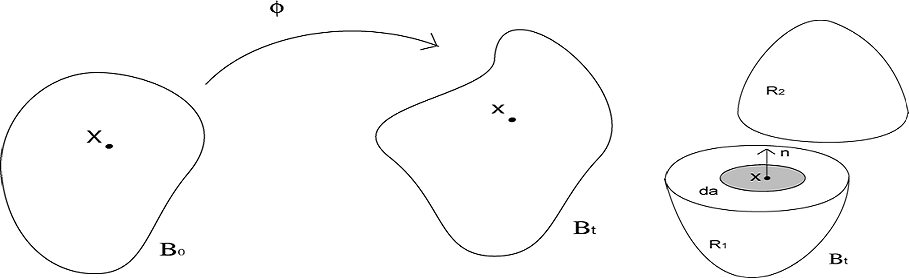
\includegraphics[width=\columnwidth]{images/continuum}
\caption{We will be solving for the mapping between the current configuration and a rest configuration. Stresses will arise via elasticity to resist changes in shape induced by this motion.}
\label{fig:phi}
\end{figure}

\section*{Basic Balance Laws}

Again, I will only present the essential details for getting started with elastodynamics. Our governing equations of motion arise from the basic principles of continuum mechanics, ultimately $F = ma$ applied over our continuum of material $\bfB_0$. This reads as:
\begin{equation*}
\rho_0 \left( \bfX \right) \frac{\partial^2 \bfu}{\partial t^2} = \nabla^{\bfX} \cdot \bfP + \bff^{\text{ext}}.
\end{equation*}
Here, $\rho_0$ is the mass density of the material, $\bff^\text{ext}$ is an externally applied force, and $\bfP$ is the first Piola-Kirchoff Stress which describes the forces of interaction in the material (specifically, $\bfP$ relates the normal of an infinitesimal surface in the material to the forces applied by one side of the material to the other; see Figure~\ref{fig:phi}). We will discuss the form of this stress in the coming sections. For now, note that it is a matrix valued function over the material:
\begin{equation*}
\bfP \colon \bfB_0 \times [0,T] \to \bbR^{2\times2}.
\end{equation*}
For elasticity, we will be relating this quantity to the deformation gradient $\bfF$. It will usually make more sense for us to consider $\bfP$ as a function of $\bfF$, but we will discuss this in the constitutive modeling section. This equation is hyperbolic and roughly like the second order linear wave equation (although the specific nature of $\bfP$ for elasticity will give rise to non-linear equations). It will be useful numerically to consider both the velocities of points of material and the displacements as unknowns. We will use $\bfv \left( \bfX, t \right) = \frac{\partial\bfu}{\partial t} \left( \bfX, t \right)$ to denote the velocity of material point $\bfX$. With this convention, we can rewrite our problem with the equivalent system:
\begin{equation*}
\begin{pmatrix}
\frac{\partial\bfu}{\partial t} \\
\rho_0 \frac{\partial\bfv}{\partial t}
\end{pmatrix}
= \begin{pmatrix}
\bfv \\
\nabla^{\bfX} \cdot \bfP + \bff^{\text{ext}}
\end{pmatrix}.
\end{equation*}

\section*{Elasticity and Constitutive Modeling}

The equations are not yet closed because we still need to determine a relationship between the stress and the state of the material. For elastic materials, this is often referred to as the constitutive or material law. Here, we will focus on hyperelastic materials. The constitutive law for such materials arises from a so-called strain energy density function $\Psi$. Specifically, we define the stress as the derivative of this energy with respect to the deformation gradient $\bfF$:
\begin{equation*}
\Psi \colon \bbR^{2\times2} \to \bbR \quad \text{and} \quad \bfP = \frac{\partial\Psi}{\partial\bfF}.
\end{equation*}
In index notation this is $P_{ij} = \Psi_{,ij}$. In general, the indices following the comma refer to partial differentiation.

The most simplistic model for elasticity is isotropic linear elaticity. In this case, we have
\begin{equation*}
\epsilon_{ij} = \frac{1}{2} \left( F_{ij} + F_{ji} \right) - \delta_{ij} = \frac{1}{2} \left( \frac{\partial u_i}{\partial X_j} + \frac{\partial u_j}{\partial X_i} \right) \quad \text{and} \quad \Psi \left( \bfF \right) = \mu \epsilon_{ij} \epsilon_{ij} + \frac{\lambda}{2} \epsilon_{kk}^2.
\end{equation*}
We are using the convention that repeated indices are summed here and $\delta_{ij}$ is the identity matrix. Differentiating this expression with respect to $\bfF$ gives us the relationship between the stress and the state of the displaced material:
\begin{equation*}
P_{ij} = \Psi_{,ij} = 2 \mu \epsilon_{ij} + \lambda \epsilon_{kk} \delta_{ij} \quad \text{or} \quad \bfP = 2 \mu \bsepsilon + \lambda \operatorname{tr}(\bsepsilon) \bfI.
\end{equation*}
This relationship between the stress and the displacement mapping is enough to close our governing system of equations. I will not give too much motivation for these equations, but note that $\bsepsilon$ is zero when $\bfF$ is skew-symmetric. Also, note that if the displacement is spatially constant, then $\frac{\partial\bfu}{\partial\bfX} = -\bfI$ and hence $\bsepsilon = \bfP = \mathbf{0}$. $\bsepsilon$ is a measure of the strain (or change of shape) in the material. Ideally, we'd like a measure that was invariant under rigid motions $\bsphi$. Unfortunately, the motions just described are only approximately rigid. The approximation is valid if we assume that the deformation is very small. In fact, we can only say that linear elasticity is valid if the deformation is very small. Otherwise, it is not a very good model. That is, it does not accurately describe any elastic materials observed in nature unless the strain is very small. A more general expression of a rigid body motion is that the deformation gradient is orthogonal. I.e., that $\bfF^T \bfF = \bfI$. In fact, more appropriate strain measures for large deformation elasticity are the right and left Cauchy-Green strain tensors: $\bfG_R = \bfF^T \bfF - \bfI$ and  $\bfG_L = \bfF \bfF^T - \bfI$, respectfully. Note that this measure is quadratic in the deformation. This will lead to nonlinear governing equations and complicate considerably the process of running our simulation. In other words, if we want to simulate large tissues that undergo significant deformation (as we would need in virtual surgery), we'll be stuck with nonlinear governing equations.

Arguably, the most simplistic model for large deformation elasticity is the \emph{Neo-Hookean} model. The hyperelastic strain energy density for such materials is given by the following equation
\begin{subequations}
\begin{equation*}
\Psi \left( \bfF \right) = \frac{\mu}{2} \left( F_{ij} F_{ji} - 2 \right) - \mu \log(J) + \frac{\lambda}{2} \log(J)^2
\end{equation*}
\begin{equation*}
\bfP \left( \bfF \right) = \mu \bfF + \left( \lambda \log(J) - \mu \right) \bfF^{-T}
\end{equation*}
\end{subequations}
where  $J$ is the determinant of the deformation gradient
\begin{equation*}
J = \det \left( \bfF \right).
\end{equation*}
The log term in this equation is there to resist changes in volume. The $\lambda$ and $\mu$ terms can be set as in linear elasticity. The most intuitive way to set these parameters is from the Young's modulus $K$ and Poisson's ratio $\nu$. This relationship is
\begin{equation*}
\lambda = \frac{K \nu}{(1 + \nu)(1 - 2\nu)} \quad \text{and} \quad \mu = \frac{K}{2 (1 + \nu)}.
\end{equation*}
The Young's modulus is a measure of the stiffness of the material and should be larger than zero (typically around $1000$ for our exercises). The Poisson's ratio is a measure of the incompressibility of the material and should be between 0 and $\frac{1}{2}$ (with $\nu = \frac{1}{2}$ being the limit of an incompressible material; note that $\lambda$ goes to $\infty$ in this case).

\begin{figure}
%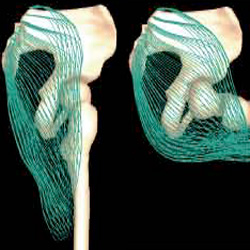
\includegraphics[width=.5\columnwidth]{images/muscle_biomechanics_2005}
\caption{Constitutive models for muscle, tendon, ligament and many other tissues must be anisotropic to accurately reflect the natural fibrous structure of these materials. In such cases, we must represent a fiber field defined over the material configuration of the material as shown above in a rectis femoris muscle.}
\label{fig:fibers}
\end{figure}

The models described so far are both isotropic. That is, the elastic response to deformation is the same regardless of which direction the material is stretched in. This is not very accurate for many fibrous tissues in the anatomy. In these cases, we need an auxiliary function $\bfg \colon \bfB_0 \to \bbR^2$ that describes the local fiber direction in the material configuration of the tissue (see Figure~\ref{fig:fibers}). The specialized response in the fiber direction can be incorporated by changing the original isotropic strain energy density to include a term based on the stretching in the fiber direction: $\bfg^T \bfF^T \bfF \bfg$. That is, the modification looks like
\begin{equation*}
\Psi \left( \bfF \right) = \Psi_{\text{iso}} \left( \bfF \right) + \Psi_{\text{fiber}} \left( \bfg^T \bfF^T \bfF \bfg \right).
\end{equation*}

\begin{figure}
%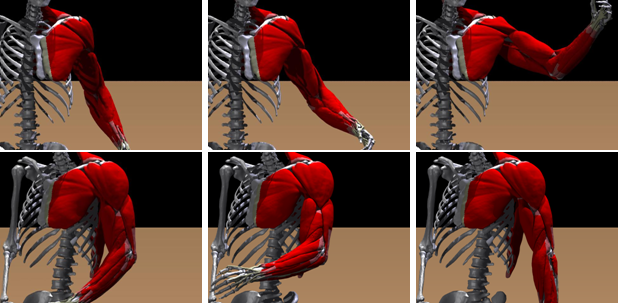
\includegraphics[width=\columnwidth]{images/muscles}
\caption{Simulation of elasticity for the musculoskeletal system.}
%\label{fig:mucles}
\end{figure}

\section*{Equilibrium and Weak Form}

We can get an idea for how to treat the spatial discretization of the partial differential equation by first considering elastic equilibrium (or quasistatic) problems where the inertial terms in the governing equations are negligible (see \cite{Teran05a} for more details). In this case we can solve directly for the displacement (i.e., we don't need to store the velocities as well). Ignoring inertia, our governing equations are then
\begin{equation*}
-\nabla^{\bfX} \cdot \bfP = \bff^{\text{ext}} \quad \text{or} \quad -P_{ij,j} = f^{\text{ext}}_i.
\end{equation*}
This can be read as the row wise divergences of the matrix $\bfP$ balance the different components of the applied forces. We'll mainly be considering \emph{finite element method} (FEM) type discretizations in these notes, so we'll look at the weak form here to get started with that. Taking a class of test functions $\bfw \colon \bfB_0 \to \bbR^2$, we take the dot product with both sides of the governing equations and integrate over $\bfB_0$ to get
\begin{subequations}
\begin{equation*}
-\int_{\bfB_0} w_i P_{ij,j} d\bfX = \int_{\bfB_0} w_i f^{\text{ext}}_i d\bfX
\end{equation*}
\begin{equation*}
-\int_{\bfB_0} \left( w_i P_{ij} \right)_{,j} - w_{i,j} P_{ij} d\bfX = \int_{\bfB_0} w_i f^{\text{ext}}_i d\bfX
\end{equation*}
\begin{equation*}
\int_{\bfB_0} w_{i,j} P_{ij} d\bfX = \int_{\partial\bfB_0} w_i P_{ij} n_j d\bfS \left( \bfX \right) + \int_{\bfB_0} w_i f^{\text{ext}}_i d\bfX.
\end{equation*}
\end{subequations}
We'd then just assume that the bottom equations hold for all suitable $\bfw$ for the weak form. Furthermore, the quantity $P_{ij} n_j$ would be supplied as a boundary condition (this would be the external loading on the material). A FEM discretization would then be done by setting up a space of interpolating functions over a mesh and considering the weak form over this finite dimensional space.

\section*{1D Elasticity}

To provide an introductory example, I will cover the case of 1D elasticity (I will assume some basic knowledge of FEM). Here, we'll first assume the material is linearly elastic. In that case,
\begin{equation*}
P(X) = \left( 2 \mu - \lambda \right) \frac{\partial u}{\partial X}
\end{equation*}
and the equilibrium equation is just Poisson's equation:
\begin{equation*}
-\left( 2 \mu - \lambda \right) \frac{\partial^2 u}{\partial X^2} = f^{\text{ext}}.
\end{equation*}
Thus, we can just use a continuous piecewise linear interpolation space of a uniform discretization of our material (which I will assume for simplicity is just some interval $(a,b)$). In this case, we will ultimately just be solving a Poisson equation for the unknown deformation field. This is only the case in 1D. If we assume that each node in the discrete domain has an associated interpolating function $N_i$, then the FEM discretized linear system is
\begin{subequations}
\begin{equation*}
A_{ij} u_j = F^{\text{ext}}_i + g_i \quad \text{where} \quad A_{ij} = \left( 2 \mu - \lambda \right) \int_a^b \frac{\partial N_i}{\partial X}\frac{\partial N_j}{\partial X} dX,
\end{equation*}
\begin{equation*}
F^{\text{ext}}_i = \int_a^b f^{\text{ext}} N_i dX, \quad g_i = N_i(b) P(b) - N_i(a) P(a)
\end{equation*}
\end{subequations}
(where we assume that $P(a)$ and $P(b)$ were already given). Now, let's consider the case of Neo-Hookean elasticity. In this case, our discretization of the weak form will give rise to a nonlinear system of equations for our displacements $u_i$:
\begin{equation*}
q_i \left( \vec{u} \right) = \int_a^b \frac{\partial N_i}{\partial X} P(F(u(X))) dX - F^{\text{ext}}_i + g_i = 0
\end{equation*}
where $u(X) = u_i N_i(X)$ (again, where repeated indices imply sumation). For Neo-Hookean materials in 1D, we have
\begin{equation*}
P(F(u(X))) = \mu \left( \frac{\partial u}{\partial X} + 1 \right) + \left( \lambda \text{log} \left( \frac{\partial u}{\partial X} + 1 \right) - \mu \right) \frac{1}{\frac{\partial u}{\partial X} + 1}.
\end{equation*}
We can think of $\vec{q} : \bbR^n \to \bbR^n$ as a nonlinear function that we need to find a zero of. We'll use Newton's method to iteratively improve our approximate solution (here, I am assuming $\vec{u}^k \in \bbR^n$ is our current approximation to the vector of discrete displacements) as:
\begin{subequations}
\begin{equation*}
\frac{\partial q_i}{\partial u_j} \left( \vec{u}^k \right) \Delta{u}_j + q_i \left( \vec{u}^k \right) = 0,
\end{equation*}
\begin{equation*}
u_i^{k+1} \leftarrow u_i^{k} + \Delta{u}_i.
\end{equation*}
\end{subequations}
The linearization of the discrete equilibrium equations can be a little tricky, so it will be good to first consider it in 1D. The general idea is to linearize the stress with respect to the deformation gradient, then linearize the deformation gradient with respect to discrete degrees of freedom.
\begin{equation*}
\frac{\partial q_i}{\partial u_j} \left( \vec{u} \right) = \int_a^b \frac{\partial N_i}{\partial X} \frac{\partial P}{\partial F} \left( F \left( \vec{u} \right) \right) \frac{\partial F}{\partial u_j} dX = \int_a^b \frac{\partial N_i}{\partial X} \frac{\partial P}{\partial F} \left( F \left( \vec{u} \right) \right) \frac{\partial N_j}{\partial X} dX
\end{equation*}
since $u(X) = u_i N_i(X)$ and $F(X) = \frac{\partial u}{\partial X}(X) + 1 = u_i \frac{\partial N_i}{\partial X}(X) + 1$. Note that the linearized system is just a spatially varying Poisson equation. However, it should be noted that for such equations we must typically require the coefficients remain positive throughout the domain. This will not always happen and can lead to difficulties with robustness. We will discuss this issue in the next section.

\begin{figure}
%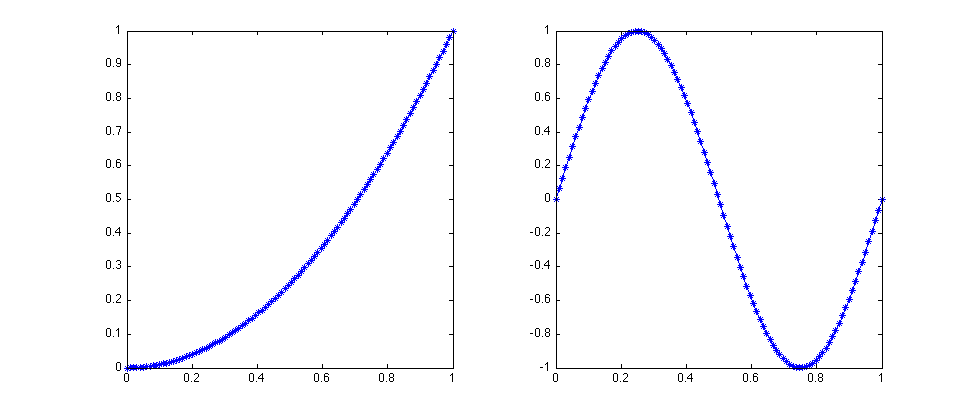
\includegraphics[width=\columnwidth]{images/elasticity_1d}
\caption{The image at the left shows an acceptable solution for the deformation $\phi$ (namely, $\phi(X) = X^2$). The solution at the right shows one that would produce inverted material (namely, $\phi(X) = \sin \left( 2 \pi X \right)$).}
\label{fig:inversion}
\end{figure}

\section*{Inversion}

The deformation mapping $\bsphi$ must be a bijection (one-to-one and onto) if we are to strictly apply the principles of continuum mechanics. This precludes many solutions you might otherwise expect to see. For example, for the 1D case, the solution must never have a derivative less than or equal to zero. I.e. many functions we are used to solving for (see Figure~\ref{fig:inversion}) are not, strictly speaking, allowable. Unfortunately, this constraint will not always be naturally achieved by our discretization. For some models (e.g. linear elasticity) it is okay that the discrete solution does not satisfy the inversion constraint. For others like Neo-Hookean, we would end up taking the natural log of a negative number. This log term is there to prevent excessive compression. However, it has the consequence that our equations become incredibly stiff under compression. Such behavior can be very problematic numerically and must be avoided in a surgical simulator. A general approach to improving robustness to discretely inverted (i.e., non-bijective) deformation mappings was developed in \cite{Irving06}. I will not go through all of the details for the sake of time. However, I will show how we can apply the principles developed in this work to our simple Neo-Hookean model.

\begin{figure}
%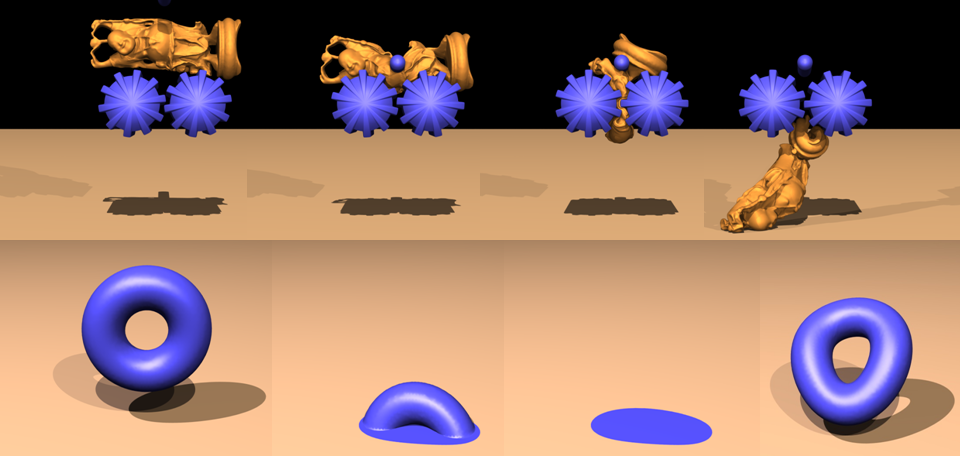
\includegraphics[width=\columnwidth]{images/buddha_gears}
\caption{These images show the the algorithm of \cite{Irving06} in action. This algorithm is based on removing the bijection constraint from continuum mechanics in the discrete setting to provide robustness to large deformation.}
%\label{fig:inversion2}
\end{figure}

The problematic term in the Neo-Hookean model is the natural log. If we replace the log with another function $r$, we can improve the robustness of our numerical simulation to inversion. This function should look very nearly like the natural log around $J = 1$ to prevent loss of accuracy, but should not have a singularity at $J = 0$. We can do this by taking $r$ to be the cubic Taylor expansion of the log around $J = 1$ (see Figure~\ref{fig:inversion3}). With this choice, we have the following expressions for the Neo-Hookean hyperelastic strain energy density and first Piola-Kirchoff stresses:
\begin{subequations}
\begin{equation*}
\Psi \left( \bfF \right) = \frac{\mu}{2} \left( F_{ij} F_{ji} - 2 \right) - \mu r(J) + \frac{\lambda}{2} r(J)^2
\end{equation*}
\begin{equation*}
\bfP \left( \bfF \right) = \mu \bfF + \left( \lambda r(J) -\mu \right) r'(J) \begin{pmatrix} F_{22} & -F_{12} \\
-F_{21} & F_{11} \end{pmatrix}.
\end{equation*}
\end{subequations}
In Figure~\ref{fig:inversion3}, we see the effect of this modification in 1D. This new model is well-defined through inversion, but accurately reflects the original model when very near the undeformed configuration. We can make further adjustments to prevent problematic values of $\frac{\partial P}{\partial F}$ (e.g. we wanted this to be positive for our 1D example). The treatment of these terms is addressed in \cite{Teran05a}.

\begin{figure}
%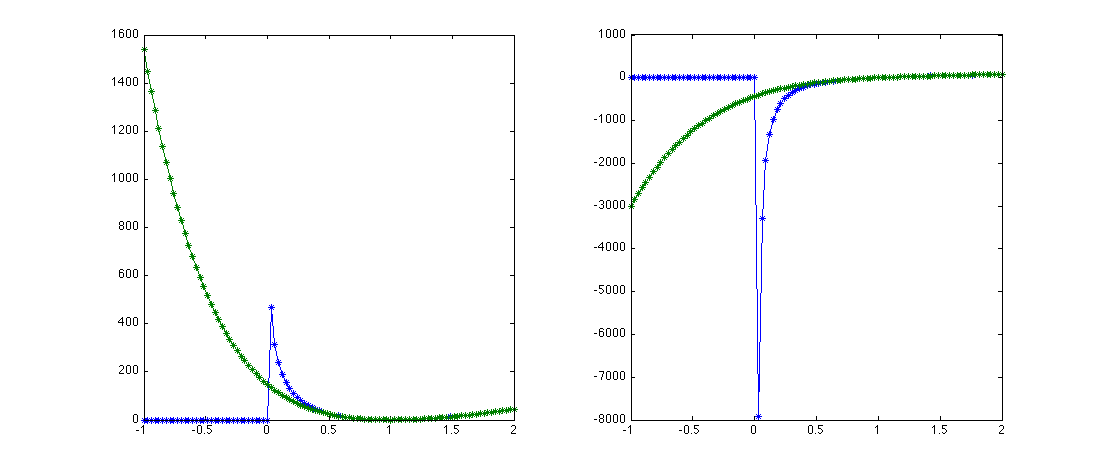
\includegraphics[width=\columnwidth]{images/invertible_neo_hookean}
\caption{The plots at the left are of the hyperelastic energy density of the 1D Neo-Hookean model. The plots at the right are of the 1D Neo-Hookean stresses. The blue curves are the unmodified Neo-Hookean model, the green curves result from replacing the log with it's cubic Taylor expansion around $J = 1$. These are preferable for the sake of robustness.}
\label{fig:inversion3}
\end{figure}

\section*{Time Stepping}

In general, our simulator will run the following loop:
\begin{equation}
\begin{array}{lc}
\text{for} \ n = 0 : N_\text{final} \\
\quad \bullet \ \text{get user boundary condition input} \\
\quad \bullet \ t \leftarrow t + \Delta{t} \\
\quad \bullet \ \text{solve nonlinear system for displacements and velocities} \\
\quad \bullet \ \text{render solution to screen}\\
\text{end}
\end{array}
\end{equation}
The key factor is that the nonlinear system must be solved in less than one thirtieth of a second to maintain an interactive simulation rate. An example of a discretization of this system that allows for inertia is the following. Let $\vec{u}^m \in \bbR^n$ represent the spatially discrete displacements at time $m$ and let $\vec{v}^m \in \bbR^n$ represent the spatially discrete velocities. We can implement backward Euler by saying
\begin{equation*}
\vec{v}^{m+1} = \frac{1}{\Delta t} \left( \vec{u}^{m+1} - \vec{u}^m \right)
\end{equation*}
and
\begin{equation*}
\rho_0 \frac{1}{\Delta t} \left( \frac{1}{\Delta t} \left( \vec{u}^{m+1} - \vec{u}^m \right) - \vec{v}^m \right) = \nabla^{\bfX} \cdot \bfP \left( \bfF \left( \vec{u}^{m+1} \right) \right) + \bff^{\text{ext}}
\end{equation*}
where we solve this final system by following a similar FEM procedure to the quasistatic case for $\vec{u}^{m+1}$. Specifically, we'd get
\begin{align*}
q^a_i \left( \vec{u}^{m+1} \right)
& = M_{ai;bj} u^{m+1}_{bj} + \Delta t^2 \int_{\bfB_0} N^a_{,j} P_{ij} d\bfX \\
& \quad {} - M_{ai;bj} \left( u^{m+1}_{bj} + \Delta{t} v^m_{bj} \right) - \int_{\partial\bfB_0} N^a P_{ij} n_j d\bfS \left( \bfX \right) \\
& \quad {} - \int_{\bfB_0} N^a f^{\text{ext}}_i d\bfX
\end{align*}
and $M_{ai;bj}=\int_{\bfB_0} N^a \rho_0 N^b \delta_{ij} d\bfX$.
